The accompanying video, \texttt{HW4\_Live\_Demo.mp4}, records live reception on the phone in the English browser interface. The original recording is 77.33 s long at 30 frames/s, with a resolution of $592\times1280$. It is retained without editing or re-encoding.

At approximately 5 s, the visible transmitter controls show a configured distance of 20 cm, $\Delta\alpha=0.1$ and a bit duration of 1 s. The receiver uses the matching bit duration. The configured distance was not independently remeasured from the screen recording. This recorded configuration supersedes the earlier guided 0.5 setting for the demo described here.

\begin{figure}[H]
\centering
\begin{minipage}{.48\textwidth}
\centering
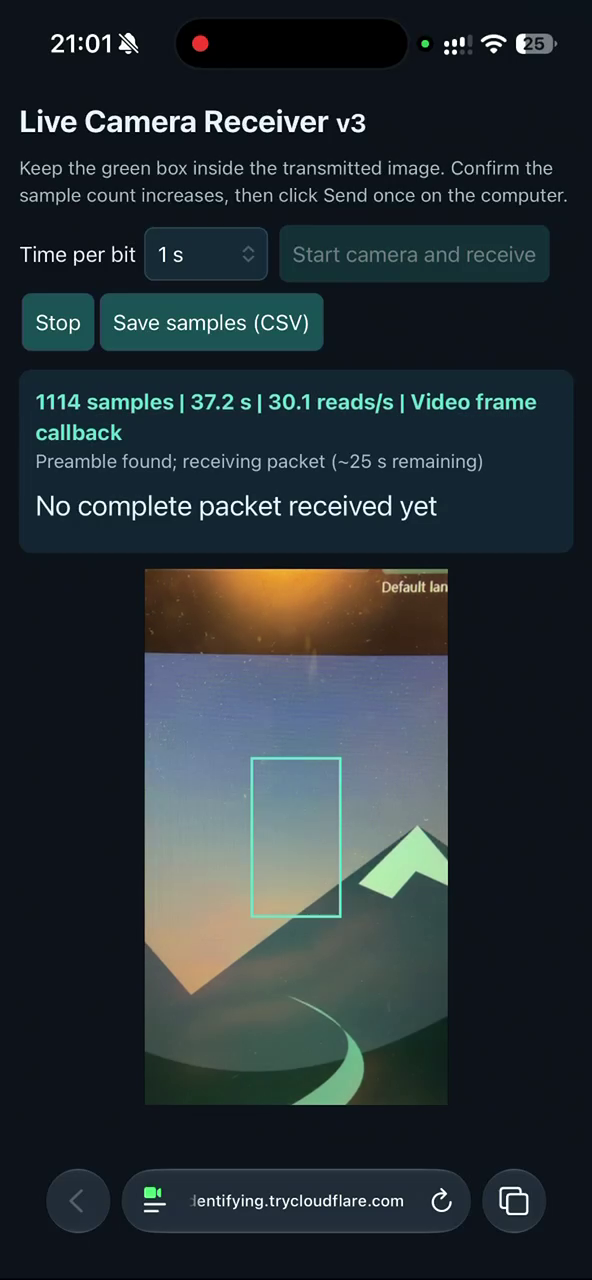
\includegraphics[height=13.1cm,keepaspectratio]{live_progress.png}
\end{minipage}
\hfill
\begin{minipage}{.48\textwidth}
\centering
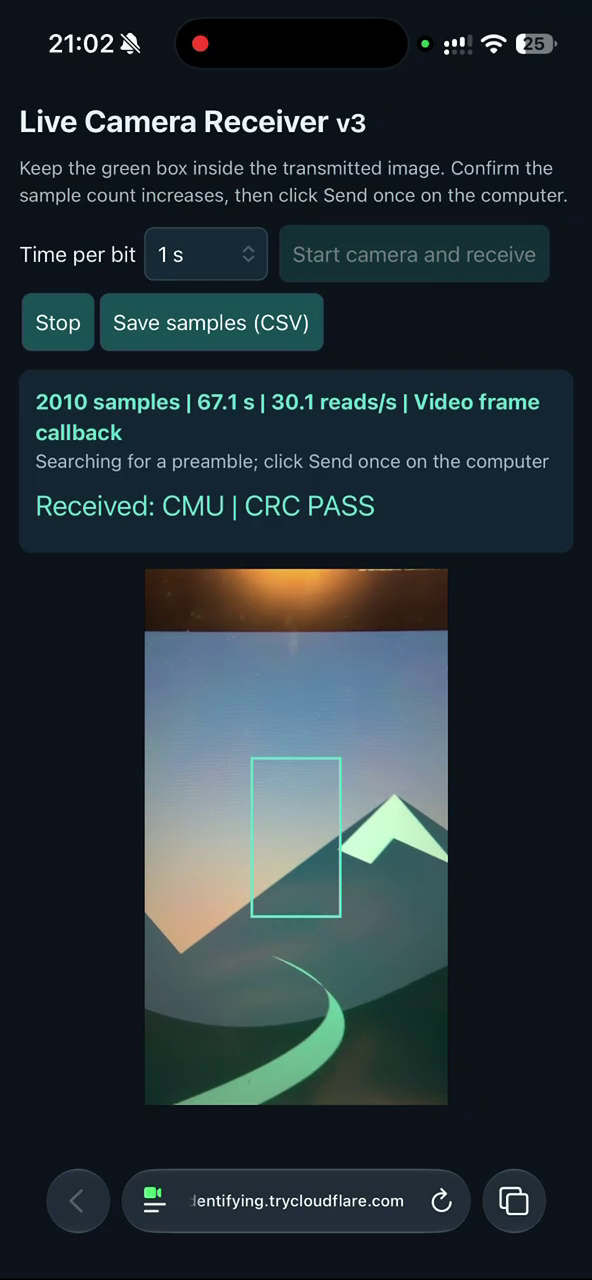
\includegraphics[height=13.1cm,keepaspectratio]{live_success.png}
\end{minipage}
\caption{Unmodified frames extracted at 40 s (left) and 70 s (right) from the supplied screen recording. Left: the receiver has found the preamble and is waiting for the rest of the packet. Right: the interface displays \texttt{Received: CMU | CRC PASS}.}
\label{fig:livedemo}
\end{figure}

The recording shows the sample count increasing and a transition from preamble detection to successful message reception. At the 70 s evidence frame, the receiver reports 2,010 samples over 67.1 s, approximately 30.1 reads/s, and video-frame-callback capture mode. These are displayed receiver diagnostics, not measurements recovered from an exported intensity trace.

The video directly documents a functional live reception, beyond the earlier participant confirmation. No raw live intensity CSV or original transmitter log for this new demo is archived. Therefore, this demo is not used to add bits to the offline BER estimates, estimate channel capacity, or infer performance at untested settings. The demonstration sends one message, \texttt{CMU}; it does not demonstrate multiple different words.
